\documentclass{beamer}
\usepackage{ctex, hyperref}
\usepackage[T1]{fontenc}

% other packages
\usepackage{latexsym,amsmath,xcolor,multicol,booktabs,calligra}
\usepackage{graphicx,pstricks,listings,stackengine}
\usepackage{textcomp}

\author{谭诗弘，黄育民，曹洪珲}
\title{智能系统设计实践}
\subtitle{六足机器人避障控制 第三次进展汇报}
\institute{武汉大学电子信息学院}
\date{2025年9月22日}
\usepackage{whu}

% defs
\def\cmd#1{\texttt{\color{red}\footnotesize $\backslash$#1}}
\def\env#1{\texttt{\color{blue}\footnotesize #1}}
\definecolor{deepblue}{rgb}{0,0,0.5}
\definecolor{deepred}{rgb}{0.6,0,0}
\definecolor{deepgreen}{rgb}{0,0.5,0}
\definecolor{halfgray}{gray}{0.55}

\lstset{
    basicstyle=\ttfamily\small,
    keywordstyle=\bfseries\color{deepblue},
    emphstyle=\ttfamily\color{deepred},    % Custom highlighting style
    stringstyle=\color{deepgreen},
    numbers=left,
    numberstyle=\small\color{halfgray},
    rulesepcolor=\color{red!20!green!20!blue!20},
    frame=shadowbox,
}


\begin{document}

\kaishu
\begin{frame}
    \titlepage
    \begin{figure}[htpb]
        \begin{center}
            
\includegraphics[width=0.2\linewidth]{pic/whulogo.png}
        \end{center}
    \end{figure}
\end{frame}

% \begin{frame}
%     \tableofcontents[sectionstyle=show,subsectionstyle=show/shaded/hide,subsubsectionstyle=show/shaded/hide]
% \end{frame}

\section{本周进展}

\begin{frame}{本周进展}
    \begin{itemize}
        \item 成功实现了对6条腿18个舵机的分别控制。
        \item 初步探索了机器人翻越障碍动作。
    \end{itemize}
\end{frame}

\begin{frame}{代码分析}
    通过类内定义的函数，能够控制它整个机器人扭矩或每一条腿的扭矩的开关，可以利用这一点实现瞬态控制。
    \begin{figure}[htpb]
        \begin{center}
            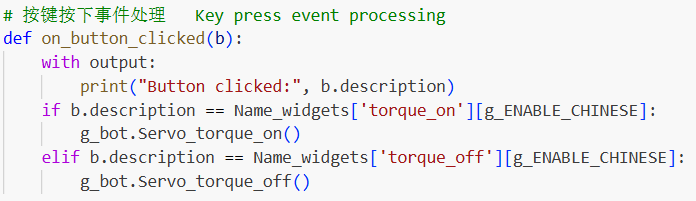
\includegraphics[width=0.8\linewidth]{pic/code1.png}
        \end{center}
    \end{figure}
\end{frame}

\begin{frame}{代码分析}
    通过滑块控件更改每个舵机的角度，即可实现对于每个舵机的精确控制。
    \begin{figure}[htpb]
        \begin{center}
            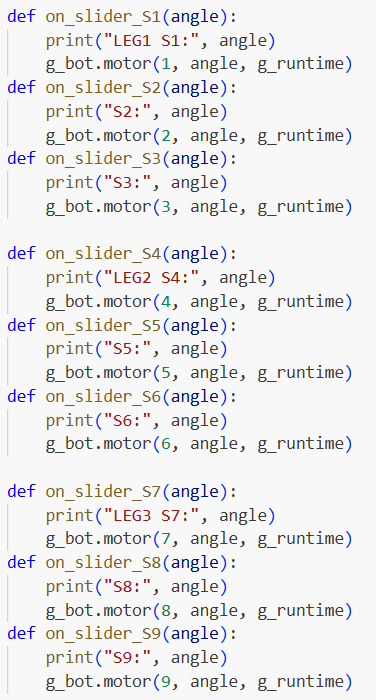
\includegraphics[width=0.3\linewidth]{pic/code2.png}
        \end{center}
    \end{figure}
\end{frame}

\begin{frame}{代码分析}
    motor(servo\_id, angle, runtime=100)：控制机器人的十八个舵机转动。

    参数servo\_id表示要控制的舵机ID号，每个舵机ID号都不同，servo\_id的取值范围为[1, 18]，分别对应机器人上的18个总线舵机。

    参数angle表示要控制舵机运动到的角度，angle的取值范围为[-90,90]。

    参数runtime为可选参数，默认值为100，表示舵机运动的时间，在有效范围内，数值越小，转动速度越快。

\end{frame}

\begin{frame}{代码分析}
    Servo\_torque\_on（servo\_id=0）:打开舵机扭矩力。

    Servo\_torque\_off（servo\_id=0）:关闭舵机扭矩力。

    可选参数servo\_id表示要控制的舵机ID号，取值范围为[0, 18]，当servo\_id=0时，表示控制所有舵机扭矩力打开或关闭；当servo\_id=[1, 18]，表示控制对应ID号舵机扭矩力打开或者关闭。

    load\_leg（leg）:打开某一条腿上的三个舵机的扭矩力

    unload\_leg（leg）:关闭某一条腿上的三个舵机的扭矩力

    参数leg表示要控制的腿ID号，leg的取值范围为[1, 6]，分别表示机器人的六条腿。 
\end{frame}

\begin{frame}{实验结果展示}
    \begin{figure}[htpb]
        \centering
        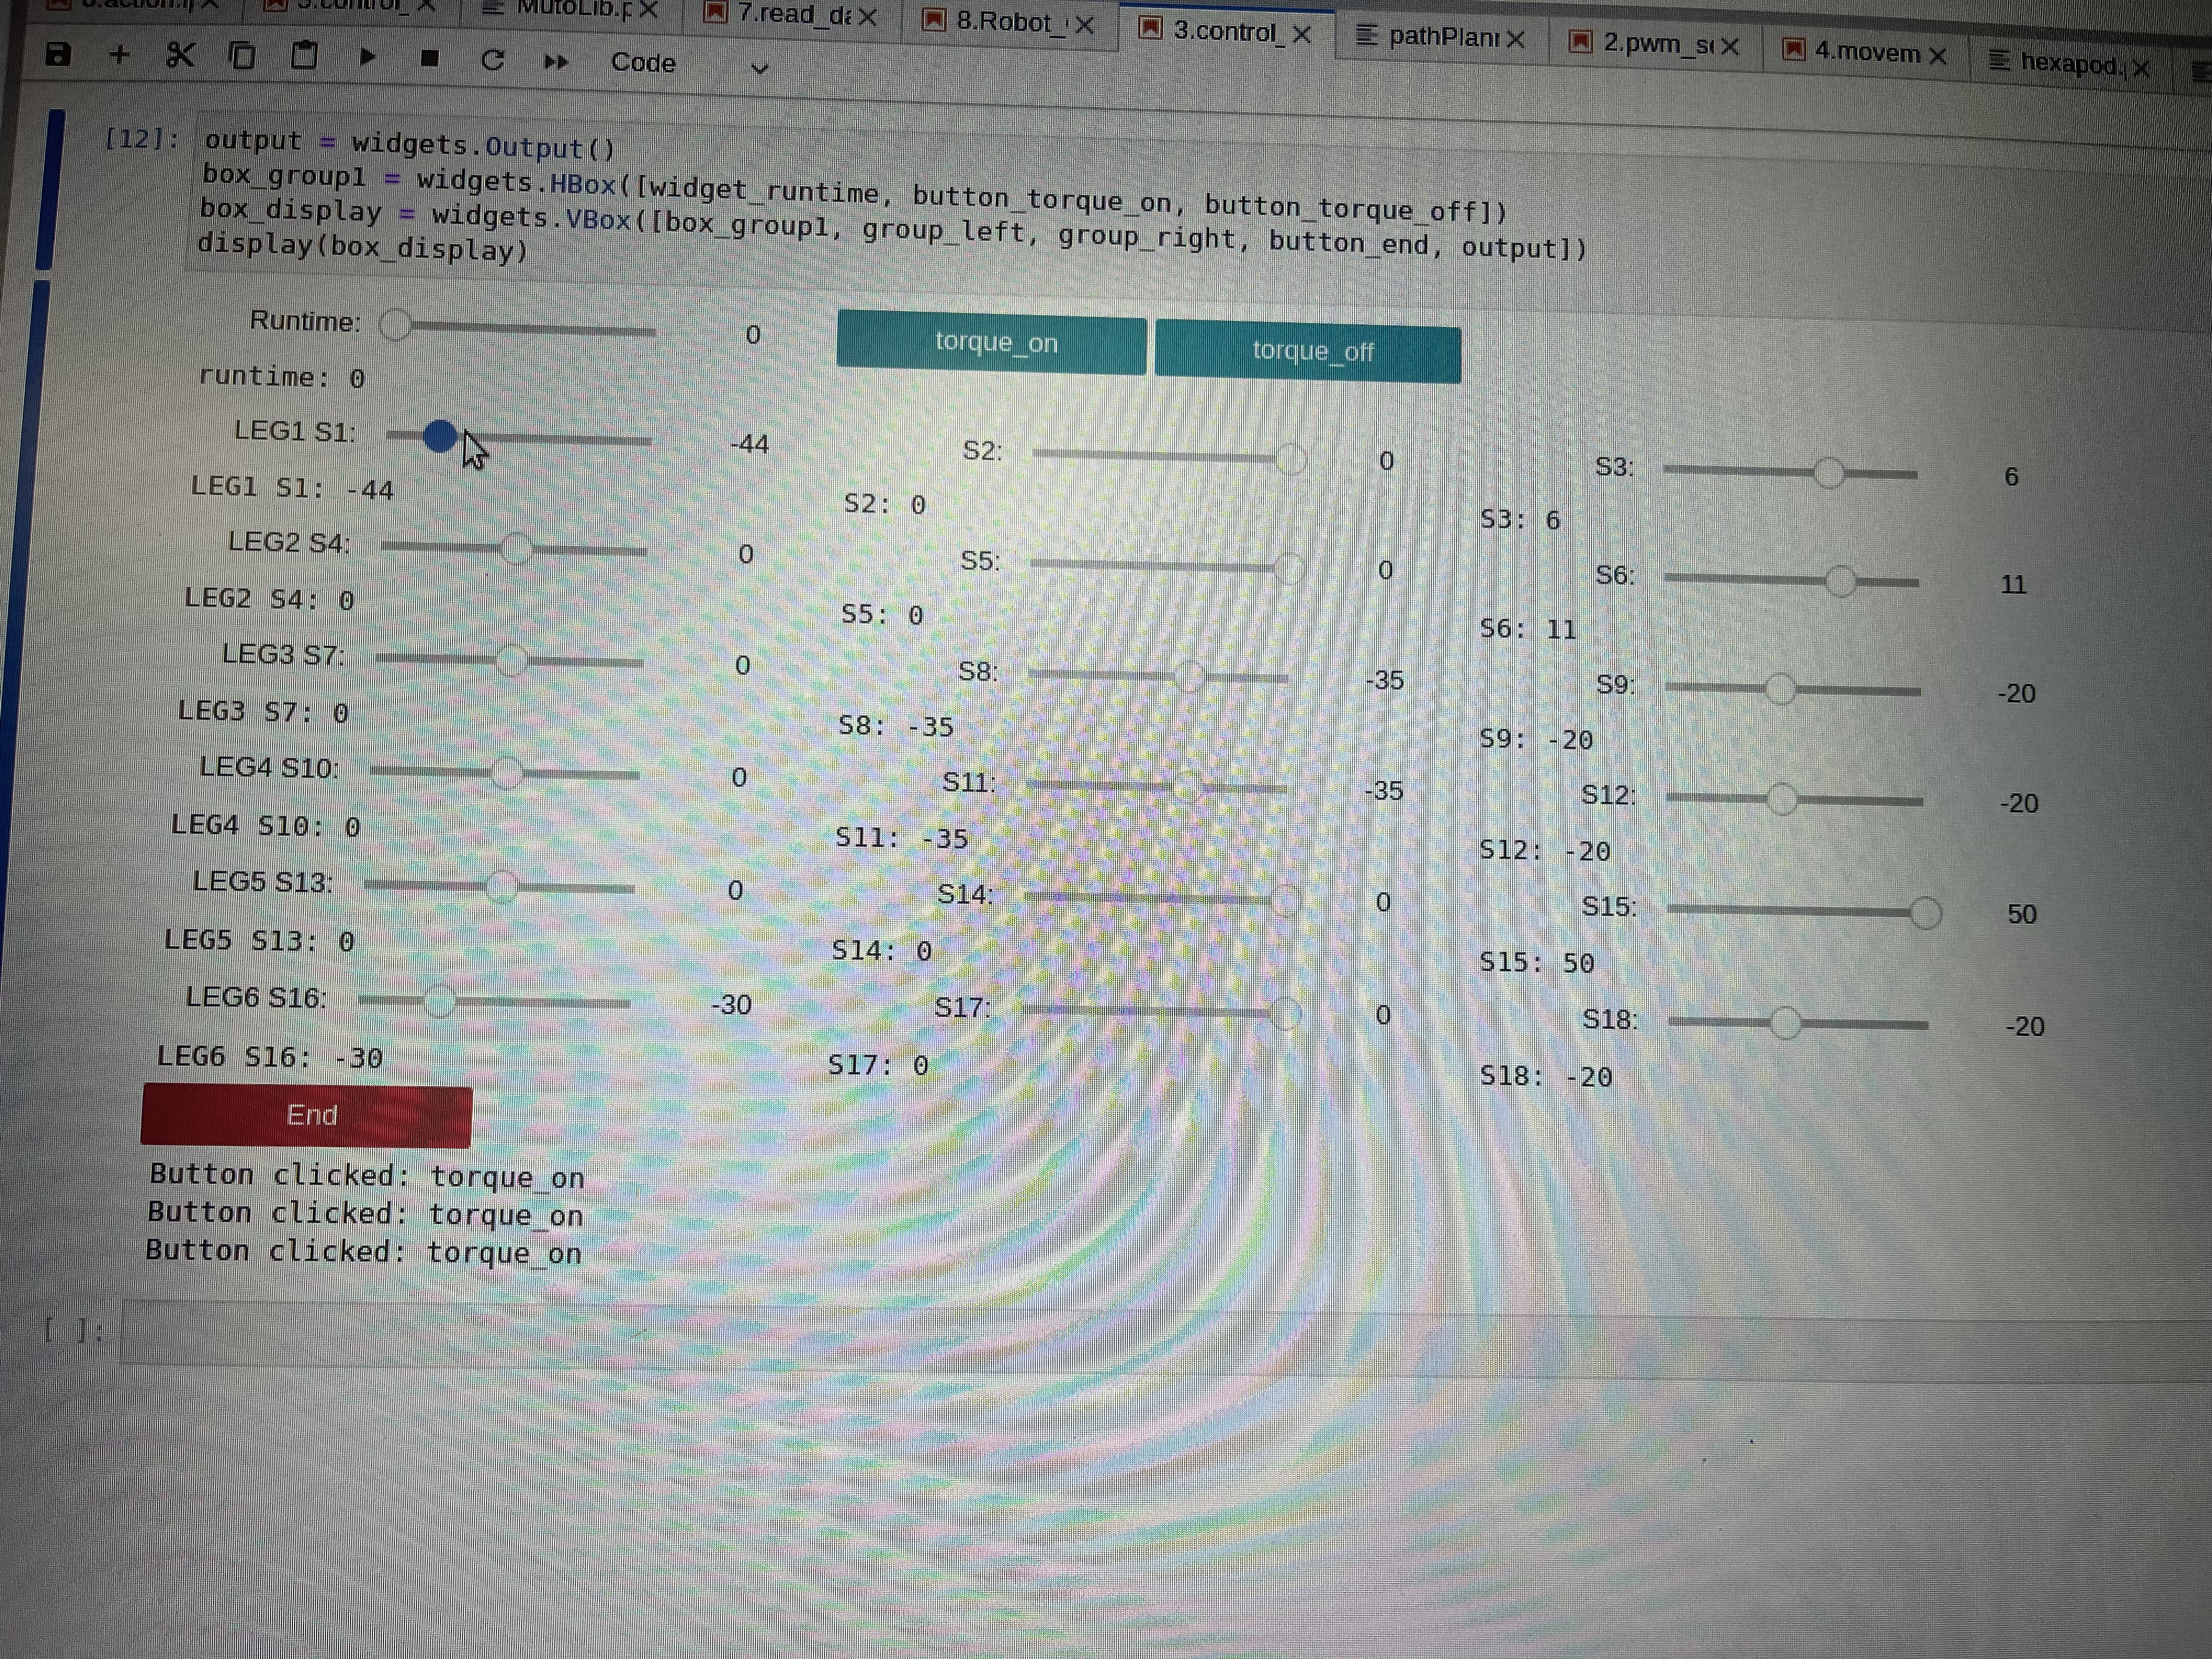
\includegraphics[width=0.8\linewidth]{pic/res.png}
    \end{figure}
\end{frame}

\begin{frame}{实验结果展示}
    \begin{center}
        视频展示
    \end{center}
\end{frame}

\section{后续规划}

\begin{frame}{后续规划}
    \begin{itemize}
        \item 现在的测试代码是通过滑块控制，通过更改空间绑定键盘或者手柄，获得更加良好的操作体验。
        \item 查询资料，给出翻越障碍方案。
        \item 给出对操作者友好的腿舵机操控方案。
    \end{itemize}
\end{frame}

\begin{frame}
    \begin{center}
        {\Huge\calligra Thanks!}
    \end{center}
\end{frame}

\end{document}